\clearpage
\section{Addition: results of the coarse breathing preview}
This addition reviews the newly submitted $32^3$, $\Delta t=0.5$ reference run, commit \texttt{b12b69c}. It uses the same equation, initial pulse, and periodic box as the main report. It is a separate calculation, not an extension of the previously reviewed $64^3$ trajectory, and no PINN was trained.
\begin{center}\small\begin{tabular}{lr}\toprule
Quantity & Recorded result\\\midrule
Target / reached propagation & $12288$ / $10321$\\
Elapsed execution time & $121.24$ seconds\\
Integration steps / reported saved frames & $20642$ / $726$\\
Maximum relative mass drift & $1.000073\times10^{-3}$\\
Maximum spectral-edge fraction & $2.65135\times10^{-6}$\\
Status & \textnormal{failed\_diagnostics}\\\bottomrule\end{tabular}\end{center}
The run stopped at the first recorded crossing of the $0.1\%$ mass-drift threshold. Mass increased numerically; this is a conservation error, not evidence of physical amplification. The spectral-edge threshold did not trigger. The complete $1500$--$2500$ observation interval was reached, as were the showcases through $10000$; $11000$ and $12000$ were not reached.
\begin{center}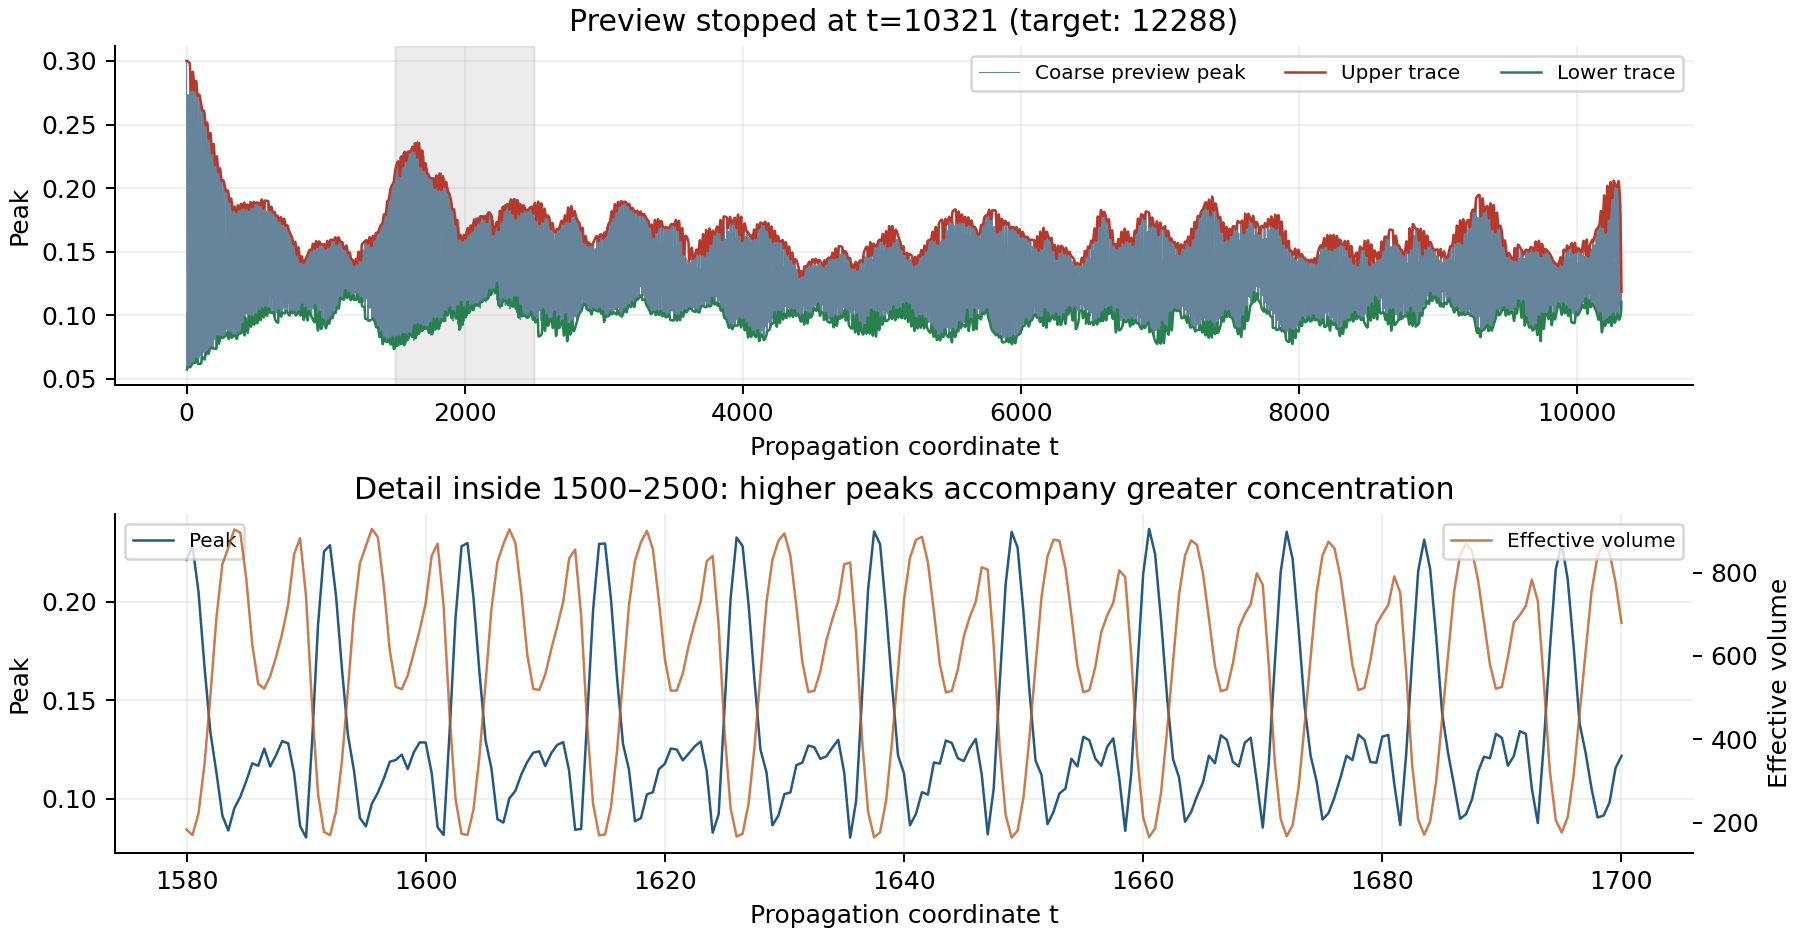
\includegraphics[width=\linewidth]{preview_results.png}\end{center}
\noindent\textbf{Preview Figure A.} The available long trajectory with upper and lower extrema traces, followed by a detail showing peak height and effective volume on separate vertical scales. Extrema traces interpolate maxima and minima in 12-unit bins and are descriptive, not rigorous bounds. The shaded interval is $1500$--$2500$.
\clearpage
\section{Concentration and thousand-point showcases}
Over $1500\leq t\leq2500$, the 2,001 diagnostic samples have peak magnitudes between $0.073723$ and $0.236918$. The effective volume
\[
V_{\mathrm{eff}}=\frac{\left(\int |E|^2\,dV\right)^2}{\int |E|^4\,dV}
\]
ranges from $164.37$ to $924.41$; smaller values indicate a more concentrated field. Peak and effective volume have Pearson correlation $-0.9134$ across this interval. This is a descriptive association between temporally dependent samples, not an independent-sample significance test or evidence of causation.

The highest recorded focus-window peak occurs at $t=1660.5$, with $V_{\mathrm{eff}}=165.17$. Thus this preview provides more evidence for repeated concentration and spreading than the peak-only data did. However, 338 of 2,001 focus samples ($16.9\%$) have at least one weak circular centroid, making the corresponding width difficult to interpret. A single coherent localized breather is not established. The effective-volume measure is independent of the centroid choice, but it too cannot distinguish all possible multi-pulse structures.
\begin{center}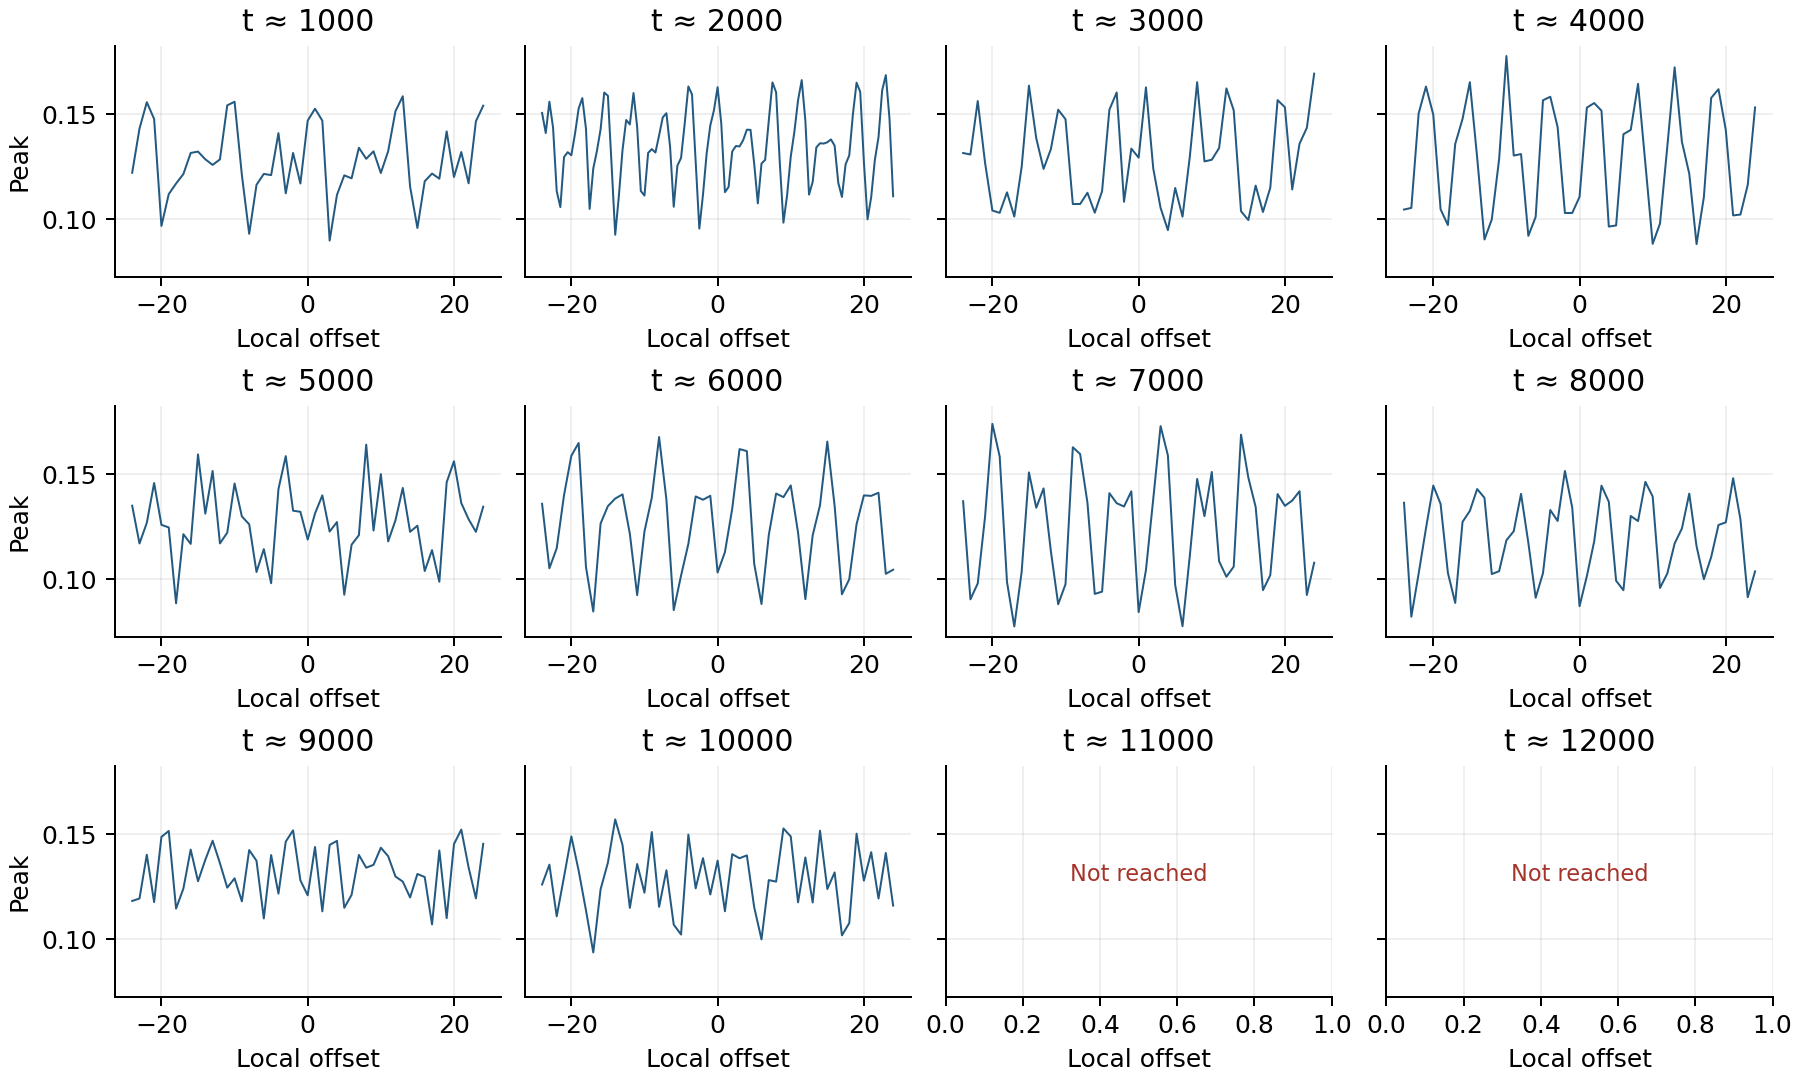
\includegraphics[width=\linewidth]{preview_milestones.png}\end{center}
\noindent\textbf{Preview Figure B.} Peak histories within $\pm24$ of each thousand. All panels share the vertical scale. These are scalar histories, not spatial pulse images; the last two requested windows were not reached.

On the common integer times $1500$--$2048$, the coarse preview differs from the earlier $64^3$, $\Delta t=0.01$ result in sampled peak by at most $1.04\%$, with mean relative discrepancy $0.223\%$. This is useful overlap agreement, but it combines grid and step changes and does not validate the complex field or the trajectory beyond $2048$. Focus-window mass drift reaches $0.0190\%$, below the operational stop threshold; passing that check alone does not establish field accuracy.

Only the summary and settings were supplied, so spatial shape, phase, and the reported field-frame files were not independently inspected. The result is a successful inexpensive qualitative preview that terminated on a numerical diagnostic, with breathing-like concentration modulation rather than a demonstrated breather or a decay law.
